\chapter{Theoretical Foundations}

\section{Sheet Metal Bending}
Sheet metal bending is a forming operation that is commonly used to produce high-volume and low-cost component in different industries. Forces are applied on the sheet metal to change it's geometry to manufacture different shapes. 
\cite[p. 1]{dib_singleensembleclassifiers_2020}
Sheet metal bending is considered complex because only the final state of the sheet metal is known, so there are many possible bending sequences which could get applied. Furthermore, the process is highly nonlinear because large deformations are applied to the sheet metal with the consequence of plastic behavior.
Conventional processes are often based on empirical trial and error approaches. \cite[p. 1]{dib_singleensembleclassifiers_2020}
A common approach is to experimentally create so named 'technology tables' which contain the bending parameters and the resulting spring back. (Quelle Hochstrate?)
This process is time and cost intensive and therefore often not suitable for the production of high-volume and low-cost components.

\subsubsection{Sheet Metal}
Sheet metal is any form of that has a relatively large length to thickness ratio, their thicknesses are typically from 0.4mm to 6mm.  % fundamentals buch 
\cite[]{baig_machinelearningprediction_2021}
Parts made of sheet metals are manufactured with different methods, such as stamping, bending, shaping etc. Bending is one of the most common methods to manufacture sheet metal parts. % manufactuing buch  \lineskip
% Anwendung sheet mal z.B. automotive

\subsubsection{Bending}
Bending is a forming operation that is used to change the shape of a sheet metal. The applied load is beyond its yield strength but below its ultimate tensile strength to achieve a permanent deformation \cite[p. 1]{baig_machinelearningprediction_2021}
During bending the metal on the outside of the neural plane is stretched and the metal on the inside of the neutral plane is compressed. The neutral plane is the plane that is perpendicular to the bending axis. \cite[p. 3]{baig_machinelearningprediction_2021}

\begin{figure}[H]
    \centering
    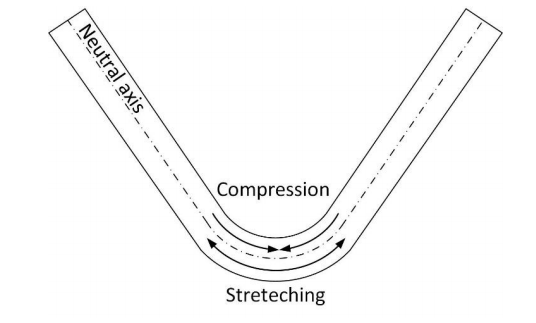
\includegraphics[width=0.6\textwidth]{neutral-plane}
    \caption{Bending plane, compression and stretching of sheet metal \cite[p. 3]{baig_machinelearningprediction_2021}}
    \label{fig:neutral-plane}
\end{figure}

\subsubsection{Air Bending}
Air bending is a variant in the V-Bending process which is performed using puch-and-die tooling. \cite[p. 416]{groover_fundamentalsmodernmanufacturing_2020} 
It is commonly used in automotive industry to manufacture sheet metal parts. \cite{kim_predictionbendallowance_2007}
In this process the punch sheet metal comes in contact of the outside edges of the die, as well as the punch tip, but it does not come in contact with the die surface. 
It is typically the preferred bending method because, its high flexibility because it is possible to achieve different bending angles using the same punch-and-die tooling.
\cite[p. 3]{miranda_formingspringbackprediction_2018}\cite[p. 1]{cruz_applicationmachinelearning_2021} 

\begin{figure}[H]
    \centering
    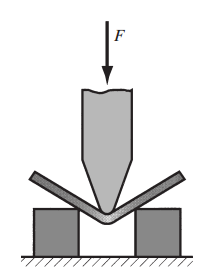
\includegraphics[width=0.3\textwidth]{air-bending}
    \caption{Air bending \cite[p. 416]{groover_fundamentalsmodernmanufacturing_2020}}
    \label{fig:air-bending}
\end{figure}

Today press brake bending machines like air bending machines are usually equipped with "copmputer numeral control" (CNC) systems that can automatically control the bending process and produce the desired shape." \cite[p. 3]{miranda_formingspringbackprediction_2018}
The air bending process is shows strong nonlinear behavior, considering its parameters and their interrelationships. \cite[p. 3]{miranda_formingspringbackprediction_2018}

\subsubsection{Spring Back} 
When the punch and therefore the bending pressure is removed at the end of the deformation operation, elastic energy remains in the bent part. This elastic energy is released and the metal sheet partially returns to its original shape. \cite[p. 113-114]{groover_fundamentalsmodernmanufacturing_2020} 

To address this issue there are several methods to compensate the spring back. For example one common method is over bending, which means that the punch angle and radius are fabricated smaller than the specified angle. 
\cite[p. 114]{groover_fundamentalsmodernmanufacturing_2020}
Prerequisite for all compensation methods is that the springback is known therefore the accurate prediction of the springback play an important role in the manufacturing process.

\begin{figure}[H]
    \centering
    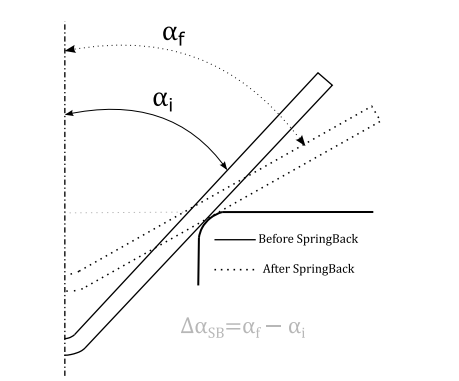
\includegraphics[width=0.5\textwidth]{spring-back}
    \caption{Spring back \cite[p. ]{cruz_applicationmachinelearning_2021}}
    \label{fig:spring-back}
\end{figure}
% \section{Bending allowance and k-factor}
% "As always, real-world materials do not behave as simply as our models. After the material has taken on its new shape in between the hardened steel tools of the press, this central neutral line will be pretty messed up by the interaction. We can’t really know the course of the neutral line after the bend without a detailed and rather complex model of the material characteristics. To make things easy, an imaginary neutral line based on a simplified approximation can be used to predict the length of the flat pattern:"
% "To do this, a correction factor, k, is introduced. The factor offsets the neutral line piece in the bend region from its center path until it has the length of the corresponding region of the flat pattern. The k-factor is empirically determined for a given material, material thickness, bend radius, and bending method. It reflects all real but unknown distortions in the bend region."

% "Since the k-factor depends on several factors, tables of empirically determined k-factors for given setups are used. Using the k-factor, we can now calculate the bend allowance "BA", which is the length of flat material that goes into the bend region. It’s simply the arc length of the "imaginary" neutral line piece, that has been offset by the k-factor:"
% "Of course, the approximation is only as realistic as the k-factor used, and it makes sense to keep your own table with k-values for the materials you intend to work with. However, the following values are a good starting point:"



% \section{Bend deduction}
% "In practice, the flat pattern length is always shorter than the sum of A and B, so everything above can be condensed in the difference between A + B and L, which is called the bend deduction "BD"." 
% \cite{by_artsciencebending_2016a}

% “Die beim Biegevorgang stattfindende plastische Formänderung beschränkt sich dabei nicht nur auf eine reine Richtungsänderung, sondern es tritt gleichfalls eine plastische Änderung der Länge auf. So wird die dem Werkzeug zugewandte Seite des Biegeteils gestaucht, während die gegenüberliegende Seite eine Verlängerung infolge Dehnung erfährt. Dieses Verhalten während des Umformprozesses wird als Biegeverkürzung oder auch als Biegezugabe bezeichnet, je nachdem, welche Seite des Biegeteils man betrachtet.” 
% \cite{rockhausen_integrationsolidworksprozesskette_2010} 

% “Dabei ist diese plastische Verformung keineswegs linear und ihre Berechnung nicht trivial. Die Biegezugabe stellt einen Zahlenwert dar, der von mehreren Faktoren abhängig ist, so zum Beispiel vom Material, von der Blechdicke und den verwendeten Werkzeugen. Zwar gibt es hierfür Formeln zu ihrer Berechnung, so zum Beispiel nach DIN 6935, doch auch diese approximieren nur die in der Fertigung tatsächlich auftretenden Biegezugaben. Daher werden oft Erfahrungswerte zugrunde gelegt, die oftmals die zuverlässigere Annäherung darstellen.” 
% \cite{rockhausen_integrationsolidworksprozesskette_2010} 

% springback is entirely intercorrelated with the stress distribution on sheet metal as residual stresses [42]. Its behavior is also affected by material properties such as strain hardening, elastic property evolution, the presence of Bauschinger effects, elastic and plastic anisotropy, and tribology between contacting surfaces [43]. Although there are mathematical models for predicting springback in bending situations, most of them are simplistic and do not take into account all influential factors.” (Cruz et al., 2021, p. 4) 

% \section{}{Machine Learning}
% "Machine learning is a branch of Artificial intelligence in which, given input data points and output value, a computer algorithm learns rules by Analyzing the data. In other words, it gives systems the ability to learn and improve themselves without explicitly being programmed. The recent advancement in technology and the development of manufacturing 4.0 also triggered the need for machine learning. It means that the machines are producing data at an unprecedented scale, so now it is needed to have fast learning algorithms that can give accurate results in a short amount of time. This need triggered engineers worldwide to build new sets of algorithms that are fast at learning and can also give reliable answers. One such group of algorithms already exist which are known as tree-based learning algorithms. A tree-based learning algorithm is a group of machine learning algorithms that are used for supervised learning."
% \cite{baig_machinelearningprediction_2021}

\section{Machine Learning}
\subsection{Ensemble Learning}
Ensemble techniques in machine learning to involve the construction of multiple models, called "learners," for a given task. The primary goal of these methods is to improve the accuracy and performance of the model by combining the predictions of multiple learners. Ensemble techniques differ from single classifier methods by constructing multiple models and combining them using a voting strategy in order to highlight different aspects of the data. This can potentially lead to improved overall performance. \cite[p. 253]{shaik_briefsurveyrandom_2019}

% "Ensembles are methods that combine multiple machine learning models to
% create more powerful models. There are many models in the machine
% learning literature that belong to this category, but there are two
% ensemble models that have proven to be effective on a wide range of
% datasets for classification and regression, both of which use decision
% trees as their building blocks: random forests and gradient boosted
% decision trees." 

% \section{Regression}

% \paragraph{Regression Genereal}

% \begin{itemize}
%     \item Explain influence of a set of variables on the outcome of another variable 
%     \item Find out which input variables are the most significant influencers of the output variable 
%     \item Identify a function that explains and predicts the value of the output variable when given the values of the input variables, therefore also called function fitting: y = f(x)
%     \item source: regression lecture 
% \end{itemize}

% Types of regression
% \begin{itemize}
%     \item Linear Regression
%     \item Logistic Regression
% \end{itemize}

% Key assumption linear relationship between input and outcome variables, but input and outcome variables can be transformed to achieve a linear relationship 

% Regression is probabilistic, not deterministic 
% – Probabilistic: Provides only expected values, based on probabilities, will include random errors 
% – Deterministic: If input variables are known, output variables can be precisely determined. Examples: Newton’s Laws in Physical sciences (Foundation of classical mechanics)

% \paragraph{Model Description}
% ...

% \paragraph{Model Evaluation} 
% Three aspects should be investigated in model evaluation of regression models: 
% – Overall accuracy and explanatory power of the model 
% – Significance of each independent variable for the outcome 
% – Confirmation of the assumptions of linear regression models

% - Accuarcy: (Mean) squared error 
% - Explanatory power (Squared correlation)

% % more in lecture 

% \section{}{ML in Bending}
% “Recently, there has been an increasing use of machine learning (ML) algorithms in various applications related to sheet metal forming to improve decision making and achieve cost-effective, defect-free, and optimal manufacturing quality [17,18]. The ML algorithms can be divided mainly in three categories: supervised learning, unsupervised learning [19], and reinforcement learning [20]. Generally, supervised learning is preferred and is used in classification or regression problems, encompassing support vector machine (SVM) algorithms, naive Bayes classifier, decision tree, the K-nearest neighbor (KNN) algorithm and artificial neural networks (ANN).” 
% \cite{cruz_applicationmachinelearning_2021}

% The authors of [21] used SVM to estimate the springback of a micro W-bending process with high prediction accuracy and generalization performance. The authors of [22] compared the performance of different machine learning algorithms (multilayer perceptron type ANN, random forest, decision tree, naive Bayes, SVM, KNN, and logistic regression) in predicting springback and maximum thinning in two different forming geometries, namely U-channel and square cup. The authors concluded that the multilayer perceptron algorithm was the best in identifying the springback, with a slightly higher score than SVM.
% \cite{cruz_applicationmachinelearning_2021}


% "The literature review shows that FEM methods and Machine Learning approaches are the two techniques that are vastly applied to predict the springback in sheet metals. Since FEM is slow so it cannot be used as an on-line tool in the production line for predicting springback [29]. In machine learning, most of the earlier attempts used artificial neural networks (ANN) to predict springback, which has several limitations. Using ANN, the predictions cannot be justified easily, i.e., the explainability of the answer from the neural network is very low. Neural networks require a lot of computation power to train the model. A neural network needs a large amount of data so that the model trained is generalized, rather than overfitted or under fitted to the data."
% \cite{baig_machinelearningprediction_2021}

% "Hence, this research article used tree-based learning algorithms which have high explainability, needs less computational power, and need less data to train the model." 
% \cite{baig_machinelearningprediction_2021}

\section{State of research}
% There is a considerable amount of literature on modeling of the
% air-bending process. Several significant references are summa-
% rized here briefly. \cite[]{kim_predictionbendallowance_2007}

% Cruz 
With the availability of data there has been an increased use of Machine Learning \ac{ML} in sheet metal forming with the goal to reduce costs and increase manufacturing quality.
\cite{bock_reviewapplicationmachine_2019} \cite[]{cao_manufacturingadvancedsmart_2019} % Quellen lesen 
The ML algorithms can be divided into the main categories supervised learning, unsupervised learning and reinforcement learning. \cite[]{liu_reinforcementlearningfreeform_2020}
Supervised learning is generally used in classification problems and regression problems while unsupervised learning is used to find patterns in data \cite[p. 2]{cruz_applicationmachinelearning_2021}.

\subsubsection*{Spring Back Prediction Using Unsupervised Learning}
Artificial Neural Networks \ac{ANN}s are widely used in sheet metal forming because of their high accuracy and generalization performance. \cite[p. 2]{cruz_applicationmachinelearning_2021} \cite[]{narayanasamy_comparisonregressionartificial_2012a} which compared regression and neural network modeling for predicting spring back of steel sheet metal during the air bending process.  
They observed that ANN was able to predict the spring back with higher accuracy. But they had a sample size of 25 and suggested further research. 
\cite[]{inamdar_developmentartificialneural_2000} developed an ANN for the air bending process to predict spring back as well as the punch travel to achieve the desired angle in a single stroke.
\cite[]{kazan_predictionspringbackwipebending_2009} developed an ANN trained with FEM simulation data to predict the spring back for the wipe-bending process.

% Therefore, the virtual tryout of sheet metal forming com-
% ponents with FEM is normally performed considering
% predefined material properties and values for some process
% parameters, such as the friction coefficient among others.
% In fact, the virtual tryout is still reliant on human expertise
% used to make key decisions at different stages of the design
% process.
% \cite[]{dib_singleensembleclassifiers_2020}

Because \ac{ANN}s need a large amount of data to train the model generating the data with real machines is a time-consuming process.
Therefore, it is common to use \ac{ANN}s trained with Finite Element Method \ac{FEM} simulation data.
\textit{Was sind die Nachteile von FEM? Warum nutze eich "echte" Experimente?}

\subsubsection*{Spring Back Prediction Using Supervised Learning}
Liu et al. (2019) used a Support Vector Machine \ac{SVM} to predict the spring back of micro W-Bending operations. \cite{liu_springbackpredictionforming_2019} 
Dib et al. (2019) compared different \ac{ML} techniques (logistic regression, SVM, KNN, ANN, random forest, decision tree, naive Bayes, MSP) to predict the spring back and the occurrence of defects in sheet metal. \cite[p. 1]{dib_singleensembleclassifiers_2020}
The authors conclude that the MLP and the SVM are the best performing algorithms and suggest further studies of ML regressions models and kriging regression models. \cite[p. 13]{dib_singleensembleclassifiers_2020}

% Artificial neural networks, among the various types of learning algorithms, are widely
% used in sheet metal forming processes due to their ability to overcome the limitations
% imposed by nonlinearities and the multiple parameters involved in forming problems.
% Several articles on air bending have been published, following the use of artificial neural
% networks [23–27]. The authors of [28] studied the use of ANN on modeling the air V-
% bending processes using both an analytical and experimental data set and demonstrated
% the capability of ANN to model the springback problem. The authors of [29] implemented
% a neural network in order to predict the stepped binder force trajectory for different punch
% displacements, in a plane strain channel forming process. The authors of [30] evaluated
% the applicability of ANN to the problem of choosing a tool geometry to bend a component
% with a defined shape. A finite element model created to simulate the bending process
% and a genetic algorithm (GA) were used to optimize the weights of an artificial neural
% network, thus reducing the deviation between the predicted tool and the experimental
% solution. The authors of [31] analyzed the performance of a multilinear regression model
% and an ANN in predicting the springback angle in air bending processes. The results
% show ANN outperforming the regression models approach for the evaluated cases. The
% authors of [32] also investigated the effect of bending and springback angles in bending
% processes. In this case, experimental data obtained from FEA models was used to design
% and train the developed ANN models. The results confirm the validity of the FEA analysis
% and consequently their capability to provide data for developing ANN. The authors
% of [33] developed a combination of error backpropagation neural network and spline
% function (BPNN-Spline) in order to estimate the springback angle in a V-die bending
% process. The results showed that the proposed BPNN-Spline model outperforms the
% traditional ANN in predicting the bending angles for different punch displacements. The
% authors of [3] developed a methodology based on ANN and FEA, capable of establishing
% the specific punch displacement for bending a sheet metal material according to the
% desired forming angle in press brake bending. The results showed that the developed
% methodology can successfully predict the required punch penetration to achieve a given
% bending angle by considering results both for geometry after springback and also geometry
% before springback.


% To the best of the authors’
% knowledge, there are currently no studies available in the
% literature regarding ML classification focused on defect
% prediction in sheet metal forming processes under vari-
% ability, which is the main subject of the current work.
% \cite[]{dib_singleensembleclassifiers_2020}




% Baig 




